\documentclass[utf8]{beamer}
\usefonttheme[onlymath]{serif}

\mode<presentation>
{
  \usetheme{Warsaw}
  \setbeamercovered{transparent}
}

\usepackage[utf8]{inputenc}
\usepackage[T2A]{fontenc}
\usepackage[russian]{babel}

\usepackage{mathtools, amssymb, bm}
\usepackage[retainorgcmds]{IEEEtrantools}

\usepackage{graphicx}
% set up graphicx to use custom path to graphs
\graphicspath{{../graphs/}}

\usepackage{tabu}
%% \usepackage{footnote}

\title[Обработка множеств логических закономерностей \insertframenumber/\inserttotalframenumber]{
  \small{
    Обработка множеств логических закономерностей с помощью
    дисперсионного критерия
  }
}

\subtitle{Выпускная квалификационная работа} % (optional)

\author[Рязанов~В.\,В., Лисяной~А.\,Е.]{
  \small{%
    \emph{Выполнил:}~Лисяной~А.\,Е. \\%
    \emph{Руководитель:}~д.ф.-м.н.,~проф.~Рязанов~В.\,В. \\%
  }
}

\institute[МГУ имени М.\,В.~Ломоносова]
{
  Факультет Вычислительной Математики и Кибернетики \\
  Кафедра Математических Методов Прогнозирования \\
  МГУ имени М.\,В.~Ломоносова
}

\date{28 мая 2015}

\DeclareMathOperator*{\argmin}{arg\,min}
\DeclareMathOperator*{\argmax}{arg\,max}

\begin{document}

\begin{frame}
  \titlepage
\end{frame}

\begin{frame}{Задачи выпускной квалификационной работы}
  \begin{enumerate}
  \item Разработка метода кластеризации логических закономерностей
  \item Построение множеств логических закономерностей небольшой
    мощности
  \item Сравнение с существующими методами на прикладных задачах
    \end{enumerate}
\end{frame}

\begin{frame}{Задача классификации}
  \begin{block}{Определение задачи классификации}
    \setlength\abovedisplayskip{0pt}
    \begin{IEEEeqnarray*}{rClCl}
    X &\in& \mathbb{R}^D &\text{ --- }&\text{пространство объектов} \\
    Y &=& \left\{1, \dots, M\right\} &\text{ --- }&
    \text{конечное множество имен классов} \\
    X^{l} &=& (x_i, y_i)_{i = 1}^{l} &\text{ --- }&
    \text{обучающая выборка}
    \end{IEEEeqnarray*}
    Построить \(a\colon X \rightarrow Y\), аппроксимирующий
    \(y^{*}(x_i) = y_i\) на \(X\).
  \end{block}
    \begin{block}{Алгоритмы решения задачи классификации}
    \begin{itemize}
    \item Метод логистической регрессии
    \item Метод опорных векторов
    \item Решающие деревья
    \item Нейронные сети
    \item Логические алгоритмы классификации
    \end{itemize}
  \end{block}
\end{frame}

\begin{frame}{Методы поиска логических закономерностей}
  \begin{block}{Определение логической закономерности}
    Пусть каждый объект выборки \(x\in X^l\) имеет размерность \(D\) и
    пусть \(\Omega\subseteq\left\{1, 2, \dots, D\right\}\). Предикат
    \[
    \varphi(x) = P^{\Omega, \bm{c_1}, \bm{c_2}}(x) =
    \bigwedge_{j\in\Omega}P^{c_1^j, c_2^j}(f_j(x))
    \]
    называется логической закономерностью класса \(K\), если:
    \begin{enumerate}
    \item \(\exists x\in K\colon \varphi(x) = 1\)
    \item \(\forall x\not\in K\colon \varphi(x) = 0\)
    \item \(\varphi(x)\) максимизирует некоторый критерий качества \(\Phi\).
    \end{enumerate}
  \end{block}
\end{frame}

\begin{frame}{Кластеризация множества логических закономерностей}
  Построенное множество логических закономерностей:
  \begin{itemize}
  \item может содержать большое количество правил
  \item может содержать похожие правила
  \end{itemize}
  Это приводит к тому, что:
  \begin{itemize}
  \item логические закономерности сложно интерпретировать
  \item по похожим правилам плохо проводить классификацию
  \end{itemize}
  \begin{block}{
      Задача кластеризации множества логических закономерностей
    }
    \begin{itemize}
      \item По исходному множеству логических закономерностей
        построить множество меньшей мощности, тем самым упростив
        задачу интерпретации полученных правил.
      \item Построенное множество должно иметь качество классификации,
        сравнимое с исходным множеством.
      \end{itemize}
  \end{block}
\end{frame}

\begin{frame}{Кластеризация множества логических закономерностей}
  Алгоритм:
  \begin{enumerate}
  \item Для каждого из \(t\) правил cоставить признаковое описание
    \begin{itemize}
    \item Вектор левых и правых границ
    \item Бинаризованное описание правил
    \end{itemize}
  \item Кластеризовать на \(k\leq t\) кластеров, найти их центры
    \begin{equation*}\label{eq:quality}
      \bm{S}^* =
      \argmin_{\bm{S}}
      \sum_{i=1}^k \sum_{\bm{z}_j\in S_i} \|\bm{z}_j - \bm{\mu}_i\|^2
    \end{equation*}
  \item По центрам кластеров построить \(k\) новых правил
    \begin{itemize}
    \item Выбрать центры кластеров в качестве новых правил
    \item Центры кластеров \(+\) критерий качества \(\rightarrow\) новые правила
    \end{itemize}
  \end{enumerate}
\end{frame}

\begin{frame}{Эксперименты и сравнение на прикладных задачах}
  \centering
  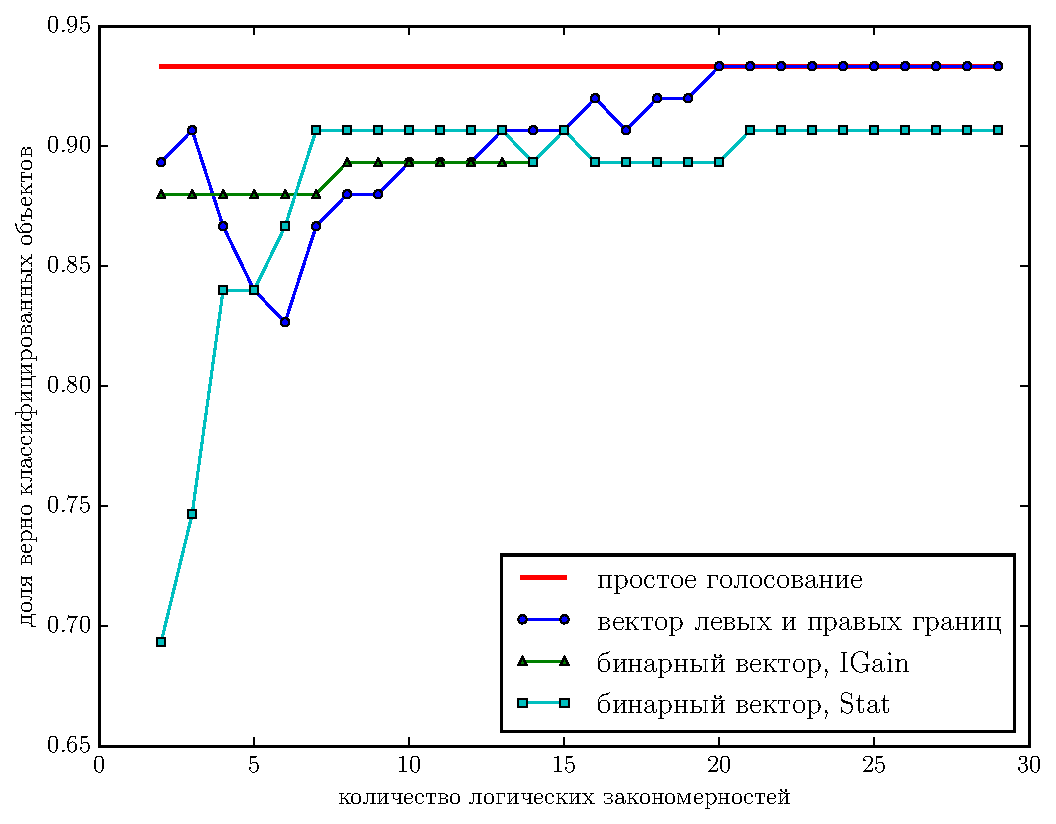
\includegraphics[width=0.8\textwidth,keepaspectratio]{iris}
  \\ Выборка <<Ирисы Фишера>>. Метод простого голосования.
\end{frame}

\begin{frame}{Эксперименты и сравнение на прикладных задачах}
  \centering
  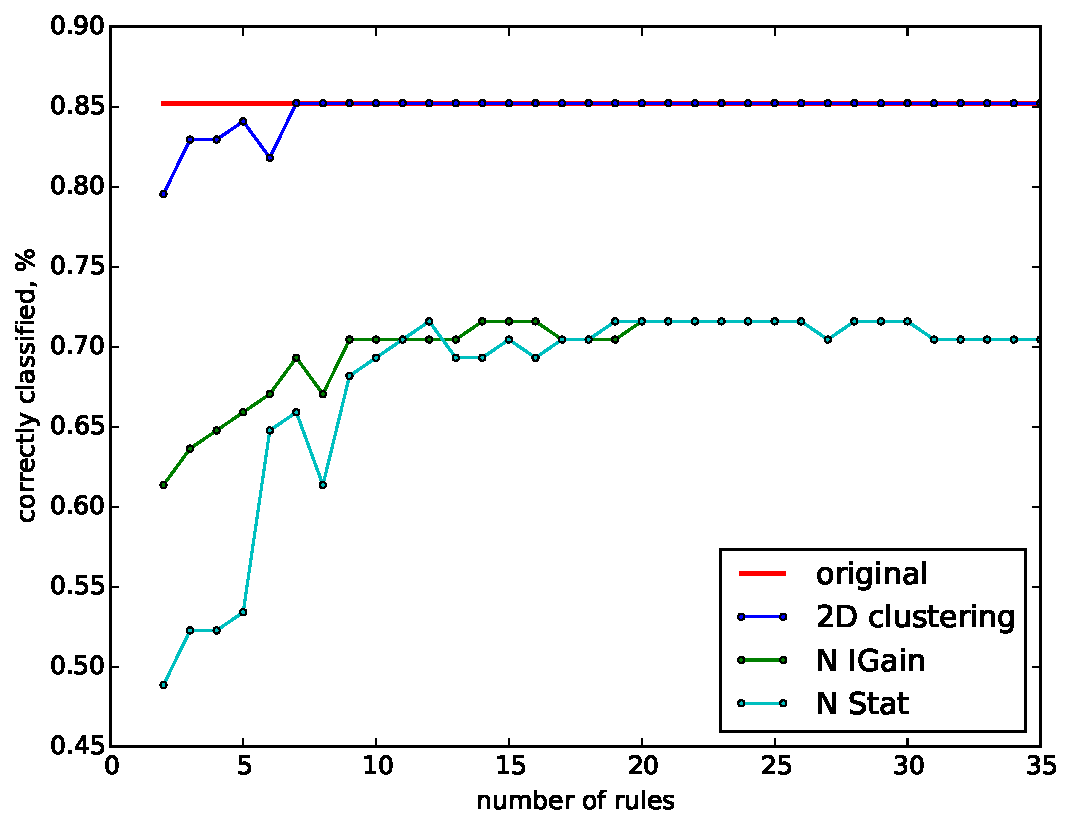
\includegraphics[width=0.8\textwidth,keepaspectratio]{wine}
  \\ Выборка <<Вино>>. Метод простого голосования.
\end{frame}

\begin{frame}{Список результатов}
  \begin{itemize}
    \item Создан метод обработки множеств логических
      закономерностей с помощью кластеризации на основе дисперсионного
      критерия.
    \item Проведено сравнение метода обработки, использующего вектор
      левых и правых границ, и метода обработки, использующего
      бинаризованное описание логических закономерностей.
    \item Экспериментально показано, что удается получить обработанное
      множество логических закономерностей с меньшим числом правил
      и сравнимым с исходным множеством качеством классификации.
  \end{itemize}
\end{frame}

\appendix
\begin{frame}[noframenumbering]{Критерии качества логических закономерностей}
  \begin{block}{Критерий Stat}
    \setlength\abovedisplayskip{0pt}
    \begin{IEEEeqnarray*}{rCl}\label{eq:stat}
      p_1,\dots, p_K &\text{ --- }& \text{верно выделяемые объекты} \\
      P_1,\dots, P_K &\text{ --- }& \text{выделяемые объекты} \\
      \text{Stat} &=& -\ln \frac{C_{P_1}^{p_1}\dots
        C_{P_K}^{p_K}}{C_l^{p_1 + \dots + p_K}}
    \end{IEEEeqnarray*}
  \end{block}
  \begin{block}{Критерий IGain}
    \setlength\abovedisplayskip{0pt}
    \begin{IEEEeqnarray*}{rCl}\label{eq:igain}
      P, N &\text{ --- }& \text{объекты из K и не из К} \\
      p, n &\text{ --- }& \text{объекты из K и не из К, выделенные правилом} \\
      H(p, q) &=& -p\log_2(p) -q\log_2(q) \\
      \text{IGain} &=&
      H\left(\frac{P}{P+N}, \frac{N}{P+N}\right)
      - \frac{p + n}{P + N}
      H\left(\frac{p}{p + n}, \frac{n}{p + n}\right) \\
      &-& \frac{P + N - p - n}{P + N}
      H\left(\frac{P - p}{P + N - p - n}, \frac{N - n}{P + N - p - n}\right)
    \end{IEEEeqnarray*}
  \end{block}
\end{frame}

\end{document}
